%%==================================================
%% chapter5.tex for BIT Master Thesis
%% version: 0.1
%% last update: Nov 8th, 2017
%%==================================================
\chapter{半参数自适应运动控制}\label{chap:5}
反馈控制是为解决实际问题而研究设计的。前面几章针对一种典型先验信息和数学描述的模型设计了半参数自适应估计与控制器,并用数值仿真验证了控制器性能。本章将考虑半参数自适应控制引入到运动控制场景,解决多关节机械臂中伺服电机的控制问题。
\section{问题描述}\label{chap:5.1}
\subsection{机器人控制}\label{5.1.1}
21世纪以来,机器人技术被认为是对未来新兴产业发展具有重要意义的高技术之一。一般来说,机器人是一个复杂的多输入、多输出非线性系统,具有时变、强耦合和非线性的动力学特征\upcite{TanWang2013}。机器人运动学和动力学的非线性和耦合性使得机器人控制系统的设计十分复杂。一般来说,将如图\ref{fig.robot}所示机器人(机械臂)的运动控制分成两个阶段分别优化,即任务空间的轨迹(路径)规划和关节空间的跟踪控制\upcite{ShinMckay1986}。前者轨迹(路径)规划部分性能的提高涉及到运动学甚至障碍物约束等多种综合因素的考量,轨迹规划器最终会以关节空间形式给后者(跟踪控制器)提供一段期望的轨迹。本章主要考虑关节空间的跟踪控制问题。

\begin{figure}[!htb]
	\centering
	\includegraphics[width=0.35\textwidth ]{ch5-ur-robot.png}\\	 % e.g.,[scale=0.75], [width=0.75\textwidth ]
	\caption{一种模块化、多关节、协作型的机器人}
	\label{fig.robot}
\end{figure}

工程应用中由于建模和测量的不准确,加上负载的变化以及外部扰动的影响,实际上难以获得机器人精确完整的运动学模型\upcite{LiuJinKun2008}。因此机器人的控制系统中存在的不确定性因素主要可以分为两类,第一类是参数不确定性,如负载质量、连杆长度、连杆质心等物理量全部或部分未知;第二类是非参数不确定性,如高频未建模动态,包括驱动器动力学、结构共振模式,以及低频难以建模动态,如动态/静态摩擦力、关节柔性等。

工业应用的机器人大多具有六个自由度,如图\ref{fig.robot}是自主研制的模块化、多关节、协作型机器人,分别由六个关节J1到J6的执行机构实现。在无障碍情形下,理论上该机器人的末端可以实现空间任意的位姿,其精度主要表现在任务空间(某个笛卡尔空间)的定位精度。工业高性能的应用场合中,一般要求机器人能达到毫米级的定位精度。机器人的位置控制问题最终要驱动各个关节的电机运动,然后经过减速器等传动机构来实现,伺服电机的运动控制与定位精度是影响机器人末端定位精度的关键因素。

\subsection{伺服电机控制}\label{chap:5.1.2}
目前大多数科研、教学和工业应用的机器人都是电力驱动的,一般可分为电压控制和电流控制两种。永磁同步交流伺服电机驱动已成为高性能伺服系统的主要发展方向。对于中小功率型机械臂(比如图\ref{fig.robot}所示的协作机器人)的电机建模来说,一般考虑电流控制情形,即电机具有如下的数学模型\upcite{LvMaster2013}:
\begin{equation}\label{eq:5.motor}
\begin{array}{c}
i_{c} = K_{a}*u_{c}\\
\tau = K_{m} * i_{c}\\
J_{0}\dot{w} + B \omega + \tau_{f}(\omega) + \tau_{l} = K_{m} K_{a} u_{c}
\end{array}
\end{equation}
其中,$Q$、$\omega$和$\dot{\omega}$分别是电机输出的角位移(单位是rad)、角速度(单位是rad/s),角加速度($\mathbf{rad/s^{2}}$);$J_{0}$是折算到电机侧的所有转动惯量之和(包括传动机构和连杆耦合值等,单位是$\mathbf{kg\cdot m^{2}}$);$B$是粘滞摩擦系数(单位是$\mathbf{N\cdot m\cdot s}$),$\tau_{f}$是Coulomb摩擦力矩(单位是$\mathbf{N\cdot m}$);$K_{a}$和$K_{m}$分别是驱动放大器的导纳系数和电机的力矩常数。

机器人多个关节同时运动时,从单个电机侧感受到的惯量$J_{0}$是时变的。虽然理论上可以通过机器人的动力学模型计算出关节侧的转动惯量值,但是前面一节介绍的不确定性因素的存在,惯量值的计算常常不准确,并且计算十分耗时。不过,经过减速器的传动,从电机侧感受到的关节侧转动惯量时变的效应减小。以一般机器人最大功率的第二个关节J2为例(减速比$G$一般为50到150之间),记该轴在机器人动力学模型中惯性矩阵所对应的值为$M_{22}$,则该轴电机侧感受到的所有转动惯量之和为
\begin{equation}\label{eq:5.J0}
J_{0} = J_{m} + \frac{1}{G^{2}}M_{22}
\end{equation}
可以看出,$M_{22}$的变化效应被缩小了$10^{4}$的数量级。然而即使这样,$J_{0$}的准取值依然难以获得。

上述伺服电机的控制输入可以认为是给定电压(本质是控制输入电流),被控的输出量是角位移或者速度。由于电机一般都是高转速、低转矩特性,并且安装位置有时和轴不在同一个地方,因此为了让电机真正驱动每个轴的运动,还需要经过减速器、皮带轮等传动机构将转速变小,同时放大转矩。除了转动惯量的不确定性外,受传动机构间隙等因素的影响,后面的摩擦力项也和角速度等具有是非线性的关系,难以精确建模。如果忽略Coulomb摩擦力矩项,借助于拉普拉斯变换,可以得到电机模型\eqref{eq:5.motor}的传递函数表述式为:
\begin{equation}\label{eq:5.trans}
\frac{\Omega(s)}{U_{c}(s)}=\frac{K_{m}K_{a}}{J_{0}s+B}
\end{equation}
其中$\Omega(s)$和$U_{c}(s)$分别是时域函数$\omega(t)$和$u_{c}(t)$的拉普拉斯变换结果。

方程\eqref{eq:5.trans}是对于速度控制是一阶模型。不过,由于机器人最终控制的是角位移,也就是速度的积分值。因此伺服电机系统可以近似为二阶线性模型,可以采用一些常规的线性控制方法,不过它的参数$J_{0}$时变,$B$常常难以知道精确值。现代伺服系统大都采用数字化离散时间控制。记采样周期为$T_{s}$,从离散时间控制角度,在第$k$个时刻电机的输入量和输出量分别记为
$$u_{k}=u_{c}(k\cdot T_{s}),\ y_{k}=\omega(k\cdot T_{s})$$
则系统\eqref{eq:5.motor}的输入输出关系可以写作
\begin{equation}\label{eq:5.nonlinear}
y_{k+1}=F(\bm{\Psi}{k},\epsilon_{k+1})
\end{equation}
其中$\bm{\Psi}_{k}$是输出$y_{k}$和输入$u_{k}$的历史数据组成的回归向量,$\epsilon_{k+1}$是随机干扰。

方程\eqref{eq:5.nonlinear}综合考虑了Coulomb摩擦等所有未建模动态,这样\eqref{eq:5.motor}转化成离散时间后不确定性大大增加,也就是说电机的离散时间模型本质是非常复杂且难以建立准确建模的,也就给直接控制系统带来了很大困难。实际上,伺服电机系统可以采用常规的线性系统方法如PID控制,可以获得一定的控制效果,但是精度和控制特性都有待提高。这从一个侧面反映了\eqref{eq:5.nonlinear}的主体是线性的,只是线性部分参数可能未知,并且含有难以建模的非参数部分。另外,伺服电机含有大量可利用的先验信息,如电机转矩的有界性、惯量变化的有界性等。这十分符合本课题前面提出的半参数系统特性。

\section{控制器设计}\label{chap:5.2}
基于前面小节的分析,本节将应用半参数模型的理论和方法分析机器人中电机运动控制问题,并设计相应的自适应控制器。
\subsection{半参数建模}\label{5.2.1}
半参数建模的目的在于建立合适的方程(包含线性和非线性部分)去描述实际系统以及蕴含的先验信息。结合方程组\eqref{eq:5.motor},电机的角速度$y_{k+1}$主要取决于上一个时刻的角速度$y_{k}$和加速度$a_{k}$。如果记$\tau_{k}$、$\tau_{k,f}$分别为电流产生的力矩和电机运动的摩擦阻力(即$B \omega + \tau_{f}(\omega)$),则电机在$k$时刻的加速度近似为
$$a_{k}=\frac{(\tau_{k}-\tau_{k,f}-\tau_{l})}{J_{0}}$$
由速度和加速度的微分关系,可以得到电机的角速度$y_{k+1}$为
\begin{equation}\label{eq:5.yk1}
\begin{split}
y_{k+1}&=y_{k}+a_{k}\cdot T_{s}+f'(\bm{\psi}_{k})+\epsilon\\
&=\theta_{1}\cdot y_{k}+\theta_{2}\cdot u_{k}+f(\bm{\psi}_{k})+\epsilon_{k+1}
\end{split}
\end{equation}
其中,$\theta_{1}$未知,可以认为近似为1,而$\theta_{2}$与电机本身参数有关,可以近似为
$$\theta_{2}=\frac{K_{m}K_{a}}{J_{0}}$$
$f(\cdot)$是未知非线性函数,主要融合了难以建模的摩擦和惯量等信息,而$\epsilon_{k+1}$是系的随机干扰。系统的控制输入为电机的电枢电流,即$u_{k}=i_{c}(k\cdot T_{s})$.

在系统\eqref{eq:5.yk1}中,$\bm{\theta}=[\theta_{1},\ \theta_{2}]$是系统的参数不确定性部分,维数
$$d_{1}=p_{1}+q_{1}=1+1=2$$
$$\bm{\phi}_{k}=[y_{k},u_{k}]$$
参数部分的先验信息表现为有界性。$\theta_{1}$近似为1,其先验信息可认为取值在0.8到1.2之间;$\theta_{1}$的上下界可以通过分析电机本身的参数$K_{a}$、$K_{m}$的合适范围,以及在机器人运动过程中惯量$J_{0}$的变化范围等数值确定大致范围。

$f(\bm{\psi}_{k})$是系统的非参数不确定性部分,回归向量$\bm{\psi}_{k}=$是历史输入输出数据的组合,即
$$\bm{\psi}_{k}=[y_{k},\ldots,y_{k-p_{2}},u_{k-1},\dots,u_{k-q_{2}+1}]$$
维数$d_{2}=p_{2}+q_{2}$不定,对应的是网络的输入层神经元个数,一般为1到10之间。一般来说,维数$d_{2}$越大,网络训练的数据越多,则逼近效果越好;但同时,过大的维数也会加重网络训练的计算量,还会造成过拟合,实际中可以调整选择合适的维数。

系统的非参数不确定性部分的先验信息也表现为有界性。由于离散时间化导致这里的$f(\cdot)$难以直接找到它的变化范围,与前面第三章和第四章的上下界函数有所不同。不过,由于电机本身功率、机械条件和加速度的制约,电机的速度与前一个时刻相差不会很大,往往在一定范围内波动,可以认为$f(\bm{\psi}_{k})$关于回归向量$\bm{\psi}_{k}$满足Lipschitz条件。具体表现为,对于两个不同的时刻$k$和$s$,$k\neq s$,存在正常数$L_{f,1}>0$和$L_{f,2}>0$,使得
\begin{equation}\label{eq:5.flim}
\begin{array}{c}
|f(\bm{\psi}_{k})-f(\bm{\psi}_{s})|\leq \Delta_{k,s}\\
\Delta_{k,s}=L_{f,1}\cdot\|\bm{\psi}_{y,k}-\bm{\psi}_{y,s}\|+L_{f,2}\cdot\|\bm{\psi}_{u,k}-\bm{\psi}_{u,s}\|
\end{array}
\end{equation}
$\|\cdot\|$记为向量的某种范数,一般为欧几里得范数。$\bm{\psi}_{y,k}$和$\bm{\psi}_{u,k}$分别是$f(\cdot)$的自变量$\bm{\psi}_{k}$中$y_{k}$和$u_{k}$的向量部分,而由于控制输入$u_{k}$和输出$y_{k}$可能在数量级上并不匹配,因此这里分别采用两个常数$L_{f,1}$和$L_{f,2}$来刻画。

一般来说,随机干扰序列$\epsilon_{k}$也具备有界性且独立同分布,在电机系统中一般取自某个随机均匀分布。关于随机干扰的先验信息为
$$\underline{\epsilon}\leq\epsilon_{k}\leq\overline{\epsilon}.$$

\subsection{自适应估计}\label{5.2.2}
为了实现半参数自适应控制,首先得设计自适应估计算法。由于半参数系统\eqref{eq:5.yk1}的参数部分也是二维情形,非参数部分也是有界的,可以利用其先验信息\eqref{eq:5.flim}借助设计信息浓缩算法估计未知参数。只是有所不同的是,非参数部分的有界形式有所不同,导致算法\ref{alg.ic.2d}和方程\eqref{eq:2.v}中关于直线的参数$v_{k,1}$和$v_{k,2}$的计算有所不同。下面给出具体推导过程。

当$k\geq2$,对于任意$0\leq s\leq k-2$,由约束关系\eqref{eq:5.flim}可以得到
\begin{equation}\label{eq:5.flim.s}
|f(\bm{\psi}_{k-1})-f(\bm{\psi}_{s})|\leq \Delta_{k-1,s}
\end{equation}
而
\begin{equation*}
\begin{split}%
|f(\bm{\psi}_{k-1})-f(\bm{\psi}_{s})|&=(y_{k}-\bm{\theta}^{\tau}\bm{\phi}_{k-1})-(y_{s+1}-\bm{\theta}^{\tau}\bm{\phi}_{s})\\
&=(y_{k}-y_{s+1})-\bm{\theta}^{\tau}(\bm{\phi}_{k-1}-\bm{\phi}_{s})
\end{split}
\end{equation*}
再结合\eqref{eq:5.flim.s}得到
\begin{equation}\label{eq:5.}
|\bm{\theta}^{\tau}(\bm{\phi}_{k-1}-\bm{\phi}_{s})-(y_{k}-y_{s+1})| \leq \Delta_{k-1,s}
\end{equation}
因此进一步得到线性约束不等式组
\begin{equation}\label{eq:5.theta.lim}
(y_{k}-y_{s+1})-\Delta_{k-1,s}\leq\bm{\theta}^{\tau}(\bm{\phi}_{k-1}-\bm{\phi}_{s})\leq\Delta_{k-1,s}+(y_{k}-y_{s+1})
\end{equation}

在几何上,式子\eqref{eq:5.theta.lim}就代表了二维空间中两个半平面的约束,作为每个周期的参数信息集$I_{k}$,可以用来设计信息浓缩估计算法。对于时刻$k-1$,可以和之前每个时刻比较得出一组类似\eqref{eq:5.theta.lim}的不等式约束,那么从理论上说存在$k-2$组。但是考虑到计算量的限制,一般情况下,只需要比较相邻两个时刻即可获得比较充分的信息关系,从而在较短时间内获得未知参数比较准确的估计值$\hat{\bm{\theta}}$。即利用$s=k-2$时的不等式约束
\begin{equation}\label{eq:5.theta.lim}
(y_{k}-y_{k-1})-\Delta_{k-1,k-2}\leq\bm{\theta}^{\tau}(\bm{\phi}_{k-1}-\bm{\phi}_{k-2})\leq\Delta_{k-1,k-2}+(y_{k}-y_{k-1})
\end{equation}

在获得$\bm{\theta}$的估计值之后,则剩余的非参数部分
$$\hat{z}_{k}=y_{k+1}-\hat{\bm{\theta}}^{\tau}\bm{\phi}_{k-1}$$
可以用第四章的基于单隐层神经网络的ITF-OELM算法逼近和预测得到$\breve{z}_{k}$的值。神经网络的输入是包含系统输入和输出历史数据组成的回归向量,实际过程中可以调整相应维度的大小。对于电机模型,一般选择1-3个输出和1-3个控制输入。选择过多的历史数据,也无太大意义,因为运动角度、角速度一般跟加速度、加加速度(有时称之为冲击)关联度较大。

\subsection{控制器设计}\label{5.2.3}
本章要解决的是机器人运动过程中关节空间的角度跟踪控制问题,从轨迹规划器得到伺服电机转动的角度之后,需要作插补运算可以得到电机在每个周期运动的角度、速度和加速度值。本章针对电机运动的角速度,从离散时间角度针对半参数模型\eqref{eq:5.yk1}设计自适应估计与控制律。在离散时间控制中,控制输入只在每个控制周期改变一次,并且只能采用得到每个周期的系统状态变量和观测值,而实际的被控对象是连续时间的模拟量。

通过相关的轨迹发生器可以得到电机在每个运动周期时刻期望的角度$Q_{k}^{*}$、角速度$\omega_{k}^{*}$和角加速度$\dot{\omega}_{k}^{*}$。为了提高伺服电机的定位精度,在电机速度控制的基础上加入位置反馈,将角度跟踪误差作为速度前馈值加入到轨迹规划产生的速度期望值中,即期望的速度跟踪值为
$$y_{k+1}^{*}=\frac{Q_{k}^{*}-Q_{k}}{T_{s}}+\omega_{k+1}^{*}$$
然后对于系统\ref{eq:5.yk1},采用必然等价原理设计的半参数自适应控制律为
\begin{equation}\label{eq:5.uk}
u_{k} = \frac{1}{\hat{\theta}_{1}}(y^{*}_{k+1}-\hat{\theta}_{2}y_{k}-\breve{z}_{k})
\end{equation}

因此,可以得到用半参数自适应控制解决电机伺服控制的总体框图\ref{fig.control.motor}。其中,$Q_{0}$和$Q_{d}$分别为电机的初始角度值和期望的角度值。
\begin{figure}[!htb]
	\centering
	
\includegraphics[width=0.85\textwidth ]{ch5-control-fig.png}\\	 % e.g.,[scale=0.75], [width=0.75\textwidth ]
	\caption{基于超限学习机的半参数自适应控制在电机运动控制中的总体框图}
	\label{fig.control.motor}
\end{figure}

\section{仿真实例}
本节以图\ref{fig.robot}所示的机器人第二轴J2安装的伺服电机控制为例验证本章设计的半参数自适应运动控制算法的性能。该伺服电机属于日本松下A6系列全数字式交流伺服电机,具体型号为MHMF022L1V2M,是一种小功率的交流同步电机。相关参数如表\ref{tab:motor}所示。
\begin{table}
\centering
\caption{电机相关参数}\label{tab:motor}
\begin{tabular*}{0.9\textwidth}{@{\extracolsep{\fill}}ll}
\toprule
项目&参数\\
\midrule
额定转矩($N\cdot m$)&0.64\\
最大转矩($N\cdot m$)&2.23\\
额定转速($r\cdot min^{-1}$)&3000\\
额定转速($r\cdot min^{-1}$)&6500\\
额定电流(A)&1.4\\
最大电流(A)&4.3\\
转矩常数$K_{m}$($Nm\cdot A^{-1}$)& 0.4571\\
电机惯量($kg\cdot m^{2}$)&$0.31\times10^{-4}$\\
谐波减速比&120\\
\bottomrule
\end{tabular*}
\end{table}

设定关节轴J2的初始值和期望终值分别为
$$Q_{0}=-45^{o}=0.524rad,\ Q_{d}=85^{o}=1.484rad$$
经过减速器之后,对应的电机角度的初始值和期望终值分别为(弧度制)
$$Q_{0}=-62.88,\ Q_{d}=178.08$$
本章用五次多项式插值作为图\ref{fig.control.motor}的轨迹发生器中的轨迹规划算法,可以做到机器人在关节空间的加速度连续且可导,其导数加加速度(冲击)连续,其轨迹比较平滑\upcite{LiuPhD2009},一般机器人控制器的关节空间的插补都是采用五次多项式进行。在仿真过程中,可以借助于机器人相关工具箱里提供的函数完成插值规划部分。

目前广泛采用的机器人电机驱动通信总线是工业实时以太网EtherCAT,其控制周期一般为0.5ms到10ms之间。为了接近实际情况,本章的电机控制周期取为$T_{s}=1$ms。采用前面设计的半参数自适应控制算法对电机的运动进行轨迹跟踪控制,事先对于电机如表\ref{tab:motor}所示准确参数未知,只是知道大致范围,在这种情况下检验控制性能。最终得到电机系统的输出结果为图\ref{fig.sim.semi.yye},以及过程中的控制输入和非线性部分的估计曲线如图\ref{fig.sim.semi.a}所示。轴2在运动过程中关节角度的跟踪误差平均值为$0.0021$rad。对于如图所示的机器人一般的运动过程中的臂长为1m,则机器人末端的跟踪误差$e_{ac}=0.0021m=2.1mm$,跟踪精度在毫米数量级。

\begin{figure}[!htb]
	\centering
	\subfigure[第二轴的关节运动速度曲线(经过减速器之后)]{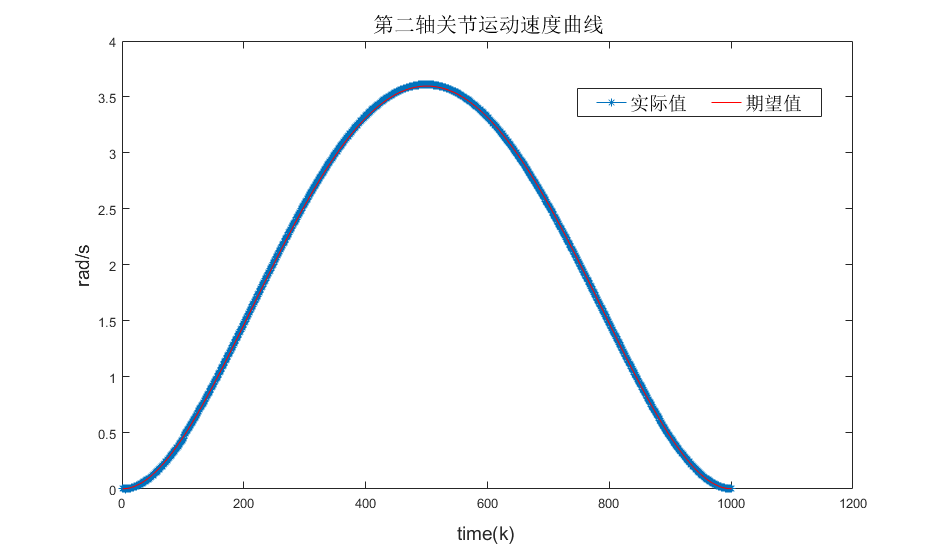
\includegraphics[width=0.65\textwidth ]{ch5-semi-omega.png}\label{fig.sim.semi.y}}\\
	\subfigure[第二轴的关节角位移曲线(经过减速器之后)]{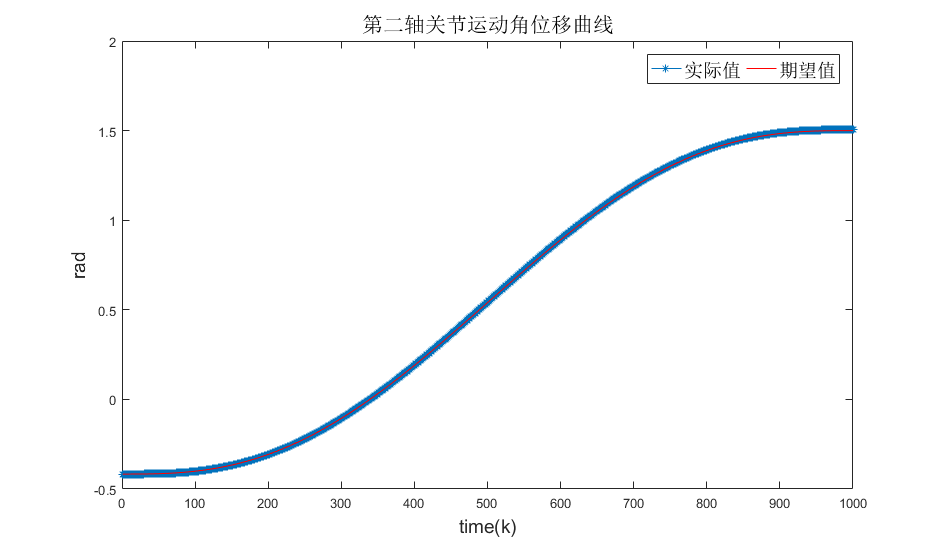
\includegraphics[width=0.65\textwidth ]{ch5-semi-Q.png}\label{fig.sim.semi.ye}}
	%\subfigure[控制输入]{\includegraphics[width=0.5\textwidth ]{ch4-sim-elmu.png}\label{fig.sim.elm.u}}
	\caption{半参数自适应控制算法的系统输出结果,关节角度跟踪误差的平均值为$0.0021$rad}
	\label{fig.sim.semi.yye}
\end{figure}

\begin{figure}[!htb]
	\centering
	\subfigure[第二轴电机系统的非参数部分的估计结果]{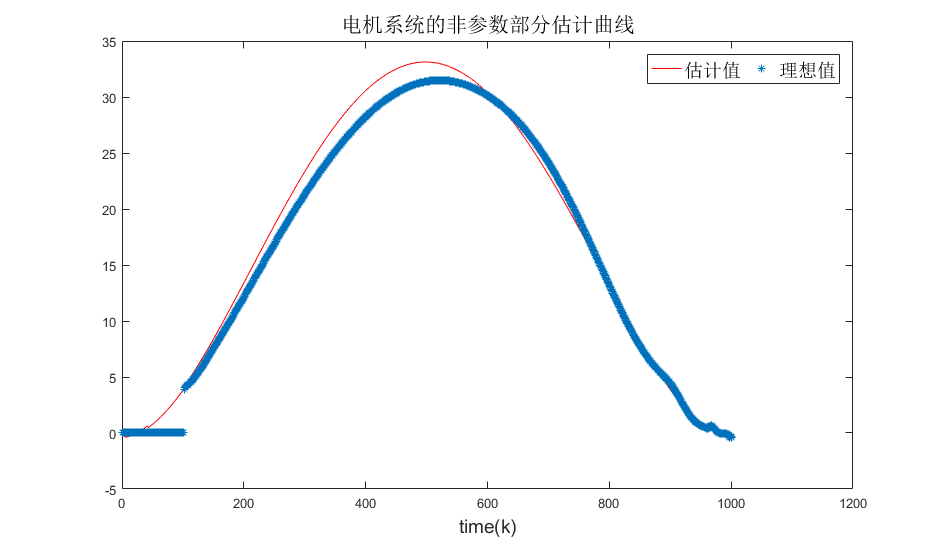
\includegraphics[width=0.65\textwidth ]{ch5-semi-f.png}\label{fig.sim.elm.f}}\\
	\subfigure[第二轴电机系统的控制输入(电机电流)变化曲线]{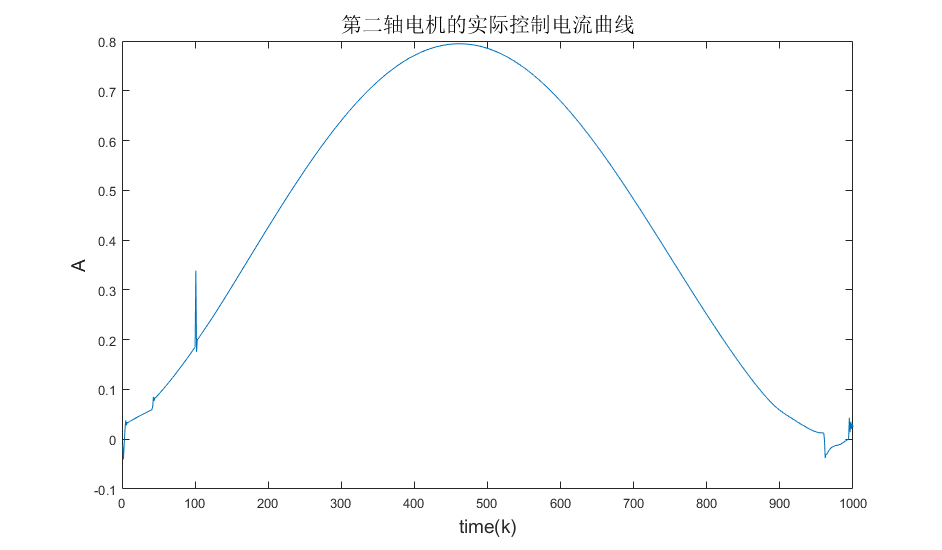
\includegraphics[width=0.65\textwidth ]{ch5-semi-u.png}\label{fig.sim.elm.u}}
	%\subfigure[控制输入]{\includegraphics[width=0.5\textwidth ]{ch4-sim-elmu.png}\label{fig.sim.elm.u}}
	\caption{半参数自适应控制算法的运行和估计特性曲线}
	\label{fig.sim.semi.a}
\end{figure}

另外,采用常规的PID算法进行对比仿真,这里采用的调试PID参数的策略是在电机空载或者小负载以及电机名义标称惯量的情况下调试得到满意的性能,然后加上在机器人负载条件下再次测试。最终得到电机系统的输出结果为图\ref{fig.sim.pid.y},以及过程中的控制输入(电机电流)曲线如图\ref{fig.sim.pid.u}所示。轴2在运动过程中关节角度的跟踪误差平均值为$0.0207$rad。对于如图所示的机器人一般的运动过程中的臂长为1m,则机器人末端的跟踪误差$e_{pid}=0.0207m=2.07cm$,跟踪精度在厘米数量级。
\begin{figure}[!htb]
	\centering
	\subfigure[第二轴的关节运动速度曲线(经过减速器之后)]{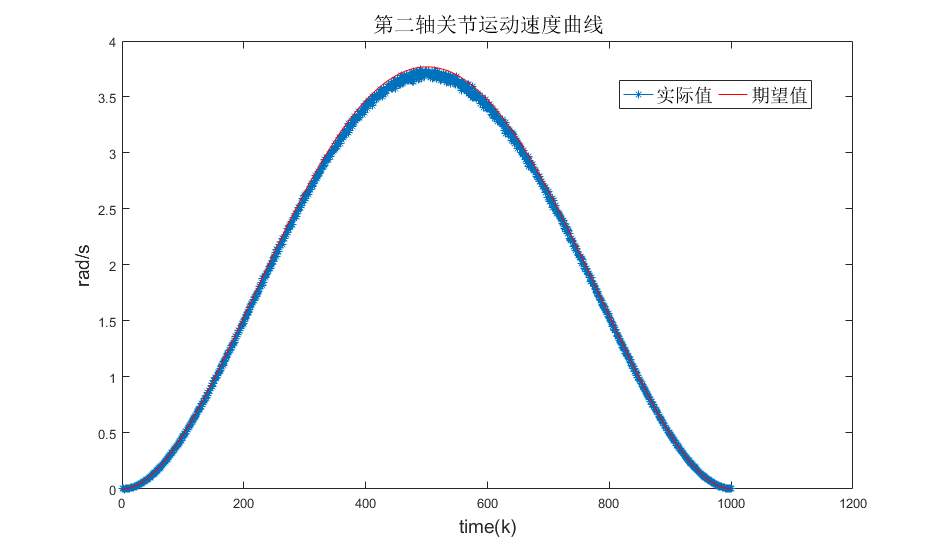
\includegraphics[width=0.65\textwidth ]{ch5-pid-omega.png}\label{fig.sim.pid.y}}\\
	\subfigure[第二轴的关节角位移曲线(经过减速器之后)]{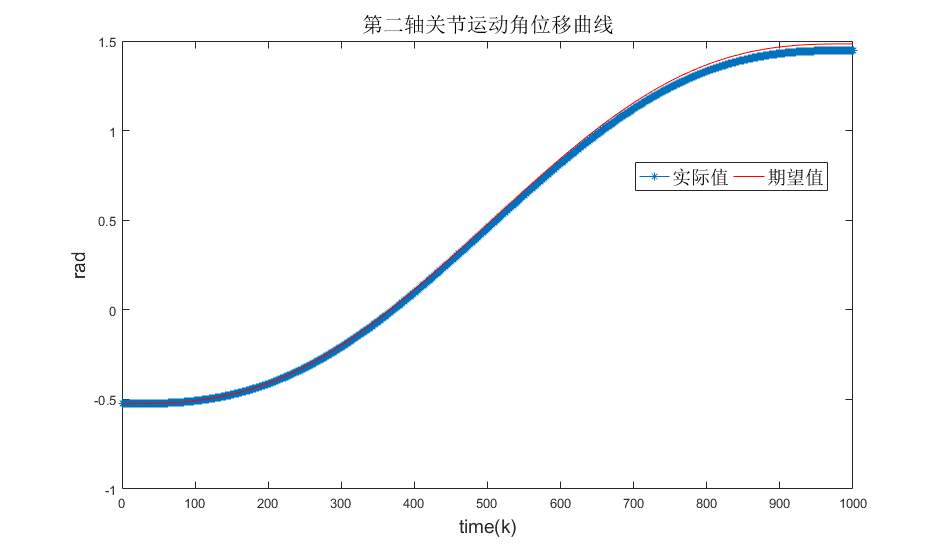
\includegraphics[width=0.65\textwidth ]{ch5-pid-Q.png}\label{fig.sim.pid.ye}}
	%\subfigure[控制输入]{\includegraphics[width=0.5\textwidth ]{ch4-sim-elmu.png}\label{fig.sim.elm.u}}
	\caption{PID控制算法的系统输出结果,关节角度跟踪误差的平均值为$0.0207$rad}
	\label{fig.sim.pid.yye}
\end{figure}

\begin{figure}[!htb]
	\centering
	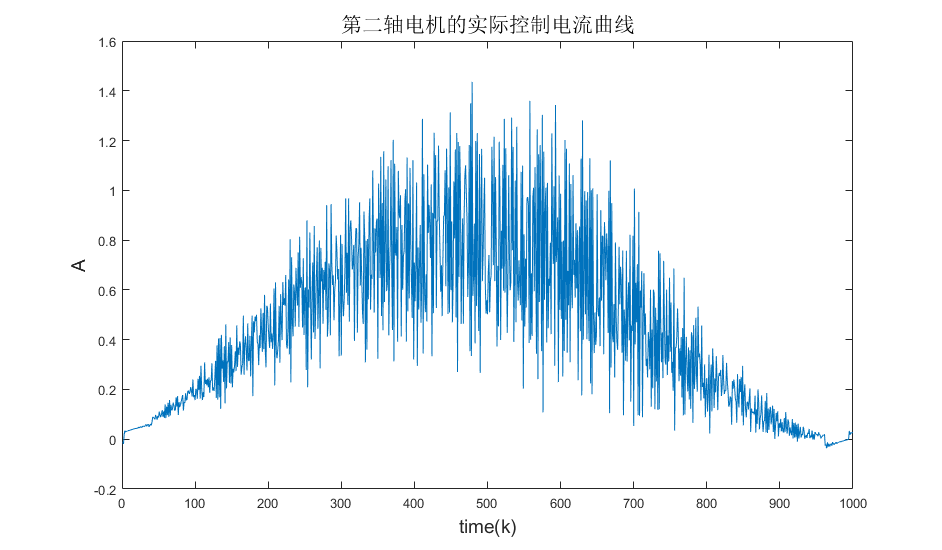
\includegraphics[width=0.5\textwidth ]{ch5-pid-u.png}\\	 % e.g.,[scale=0.75], [width=0.75\textwidth ]
	\caption{PID控制算法中第二轴电机系统的控制输入(电机电流)变化曲线}
	\label{fig.sim.pid.u}
\end{figure}

对比上面两种控制方法结果,可以得出本课题采用基于超限学习机的半参数自适应控制算法对于解决运动控制问题有如下特点:
\begin{enumerate}
\item 基于超限学习机的半参数自适应控制算法提高了系统的跟踪精度,对比常规的PID控制精度可以提高大约一个数量级(10倍)。
\item 基于超限学习机的半参数自适应控制对于系统精度提高主要来源于非参数部分的准确估计,而非参数部分的估计在一定程度也依赖于参数部分的估计。
\item 半参数自适应估计的准确性导致最终的控制输入有比较好的变化曲线,对比图\ref{fig.sim.elm.u}和\ref{fig.sim.pid.u}容易得出。
\end{enumerate}

\section{本章总结}
本章主要将基于超限学习机的半参数自适应估计与控制应用到运动轨迹跟踪控制中,解决机器人运动中电机的控制问题。首先分析了机器人轨迹跟踪和伺服电机运动控制中多种不确定性存在等控制难点;然后应用本课题提出的半参数系统对单轴伺服电机进行了分析和建模;接着设计了基于超限学习机的半参数自适应估计与控制算法应用单轴伺服电机的控制;最后设计了仿真对比实验测试和验证半参数自适应控制的性能。